\section{Группы фигур}
Рассмотрим фигуру $\Phi$ в ,,обычном`` $n$-мерном пространстве.\footnote{Мы не будем рассматривать размерности больше 3.} Группа преобразований $\Phi \to \Phi$, переводящих фигуру в себя называется \emph{полной группой фигуры $\Phi$.} Подгруппа, сохраняющая ,,ориентацию`` фигуры, называется \emph{собственной группой фигуры $\Phi$.}

\subsection{Группы диэдров $D_n$}
\begin{definition}[Группа диэдра]
    Группа преобразований правильно плоского $n$-угольика, лежащего в трёхмерном пространстве, называется \emph{группой диэдра\footnote{\emph{Диэдр (диэдра)} --- это правильный плоский многоугольник.
}.} 
\end{definition}
\begin{example}
    Простейший диэдр, пусть нам и непривычный, называется \emph{двуугольник}. Его можно представлять себе, как выпуклую линзу или глаз (на \cref{fig:D_23}). Группа $D_2$ такой линзы совпадает с группами описанного вокруг неё прямоугольника, и вписанного в него ромба. Она состоит из трех поворотов, вокруг каждой из координатных осей, а также из тождественного движения, которое еще обозначается $\id$.
\end{example}

\begin{practice}
    Убедитесь, что $D_2 \cong \Z/(2) \times \Z/(2)$.
\end{practice}

Группа $D_2$ настолько часто возникала в математике, что для нее придумали даже специальное название. А именно, \emph{Группа Клейна или четверная группа Клейна} $V_4$.

Вообще, имя Феликса Клейна не возникает в школьной программе, что и понятно. Его знаменитый доклад на \emph{Эрлангенской конференции} призывал изучать геометрию именно с помощью групп, как это делаем и мы сейчас: изучать то, какие движения оставляют на месте разные объекты.

\begin{figure}[ht]
    \begin{center}
        \begin{asy}
            size(0,40mm);
            draw((0,0).. tension 2.5 ..(2,1).. tension 2.5 ..(4,0).. tension 2.5 ..(2, -1).. tension 2.5 ..cycle, linewidth(bp));
            draw((0,0)--(2,1)--(4,0)--(2,-1)--cycle, dashed+grey);
            draw((0,1)--(4,1)--(4,-1)--(0,-1)--cycle, dashed+grey);
            draw((-0.2, 0)--(4.2,0), dashed+red);
            label("$s_1$", (4.4, 0.2), red);
            draw((2, 1.2)--(2, -1.2), dashed+blue);
            label("$s_2$", (2.4, 1.2), blue);
        \end{asy}
        \begin{asy}
            size(0,40mm);
            triangle t = triangleabc(3,3,3);
            draw(t);
            point O = circumcenter(t);
            draw(line(t.VA, O), dashed+blue);
            draw(line(t.VB, O), dashed+blue);
            draw(line(t.VC, O), dashed+blue);

            label("$s_1$", midpoint(t.BC)+(0.5,0), blue);
            label("$s_2$", midpoint(t.AC)+(-0.2,0.4), blue);
            label("$s_3$", midpoint(t.BA)+(-0.3,-0.3), blue);

            point Ha = midpoint(segment(O, t.VA)); 
            point Hb = midpoint(segment(O, t.VB)); 
            point Hc = midpoint(segment(O, t.VC));

            point Ma = intersectionpoint(line(Hb, Hc), line(t.VA, O));
            point Mb = intersectionpoint(line(Ha, Hc), line(t.VB, O));
            point Mc = intersectionpoint(line(Hb, Ha), line(t.VC, O));

            point Ta = O + O - Ma;
            point Tb = O + O - Mb;
            point Tc = O + O - Mc;

            draw(Mc..midpoint(segment(Hb, O))..Ma, red, Arrow);
            label("$r$", Hb+(-0.1, 0.3), red);

            draw(Ta..Mb..Tc, red, Arrow);
            label("$r^{-1}$", Mb+(0, 0.3), red);

            dot(O, red+3);
        \end{asy}
        \caption{Двуугольник $D_2$ и треугольник $D_3$.}
        \label{fig:D_23}\qquad
\end{center}
\end{figure}

\begin{example}
    Следующая диэдральная группа --- группа треугольника $D_3$ (на \cref{fig:D_23}). Она состоит из тождественного движения, двух поворотов $r, r^{-1}$ на $\pm 120^\circ$ вокруг центра треугольника, а также из трёх осевых симметрий $s_1, s_2, s_3$. Воспользуемся следующей леммой, что доказать изоморфизм $S_3$ и $D_3$.
\end{example}

\begin{lemma}
    Движение плоскости одозначно задается своим действием на вершины треугольника.
\end{lemma}

В этом курсе мы ее строго не докажем, но я приведу некоторые факты, которые помогут ее понять. Понятно, что действия на две вершины не хватит, ведь можно сделать осевую симметрию относительно прямой, проходящей, через этим точки. А трёх вершин уже будет достаточно, ведь мы будем знать расположение третьей, а вернее в какой полуплоскости она лежит.

\begin{proof}
    [Доказательство изоморфизма]
    Теперь можем доказать изоморфизм групп. Понятно, что $D_3 \subset S_3$. Осталось показать, что $S_3 \subset D_3$. Любой элемент из $S_3$ действует на вершины треугольника, а тем самым пораждает движение плоскости, что в частности является движением треугольника.
\end{proof}

Поскольку движение плоскости, сохращяющее правильный $n$-угольник определяется своим действием на 3 точки (какой-нибудь вершиной, напрмер, и парой соседних сторон). Тогда группа диэдра при $n \geqslant 3$\footnote{На самом деле, даже при $n \geqslant 2$.} состоит из $2n$ движений. Выбранную вершину можно перевести в любую из $n$ вершин диэдра, а потом двумя способами совместить оставшиеся ребра. Этим $2n$ движений состоят из $n$ поворотов на $\frac{2\pi}{n}$ (циклическая группа порядка $n$), а также $n$ симметрий относительно прямых проходяший через пару середин противоположных сторон, в случае четноугольника, а в случае нечетноугольника --- прямые проходящие через вершину, и середину противолежащей стороны.

\begin{practice}
    Порисовать диэдры, их оси симметрий и повороты. 
\end{practice}
\begin{practice}
    Написать таблицы Кэли (умножения) для групп $D_3, D_4, D_5$.
\end{practice}

\begin{figure}[ht]
    \centering
    \begin{tabular}{c c}
        
\includegraphics[height=3cm]{images/Mercedes-Logo.png} & 
        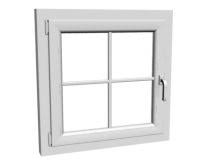
\includegraphics[height=3cm]{images/window.jpg} \\
        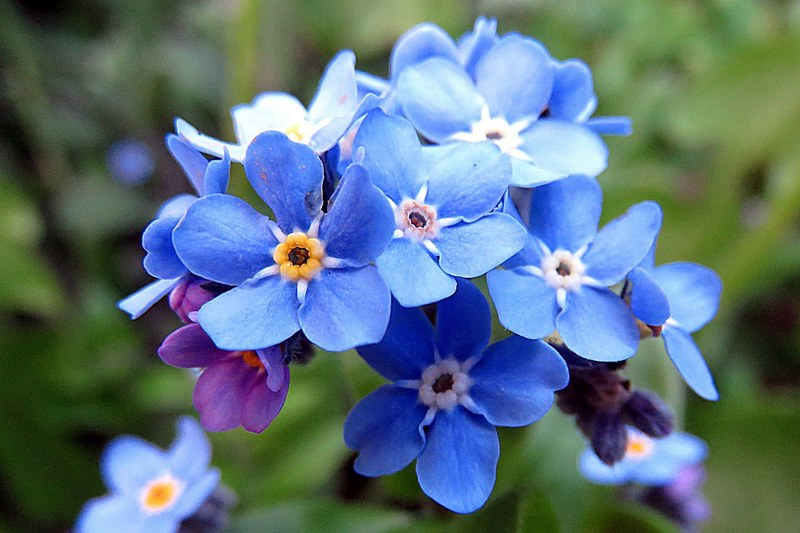
\includegraphics[height=3cm]{images/nezabudka_1.jpg} & 
        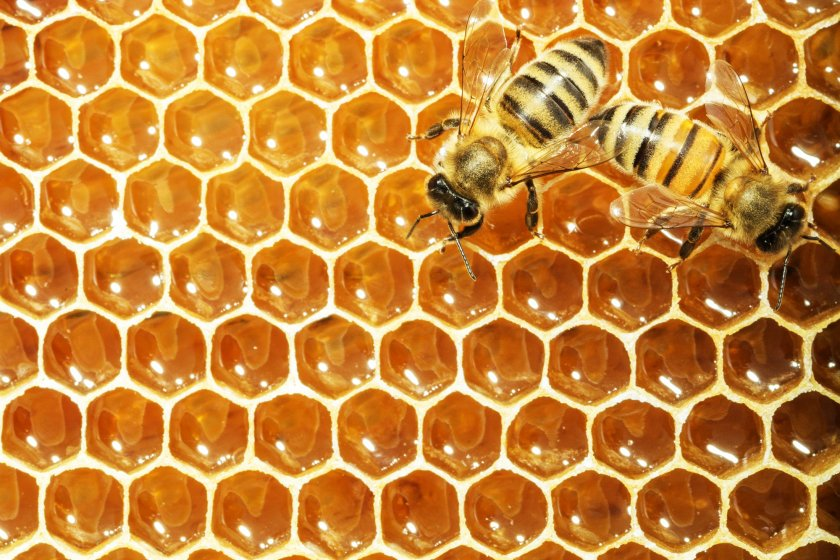
\includegraphics[height=3cm]{images/38018.pkfy9c.840.jpg}
    \end{tabular}
    \caption{Другие объектые, обладающие группами $D_3$, $D_4$, $D_5$ и $D_6$.}
\end{figure}

\subsection{Группа тетраэдра}
%TODO: вот тут мочно нужно будет наприсовать.

Как и в случае с треугольником воспользуемся схожей леммой. Тогда любое движение пространства, сохраняющее на месте тетраэдр однозначно определяется своим действием на вершины. Тем самым, полная группа тетраэдра изоморфна $S_4$.

Собственная же группа состоит из $4 \cdot 3 = 12$ движений: поворот тетраэдра однозначно задаётся своим действием на вершину, и три ребра которые через нее проходят, и может переводить эту вершину в любую из четырёх вершин, после чего, остается ровно три возможности для совмещения рёбер, сохранющее ориентацию пространства. Полный список всех собственных движений тетраэдра: 
\begin{enumerate}
    \item тождественное преобразование;
    \item $4\cdot 2 = 8$ поворотов на углы $\pm 120^\circ$ вокруг прямых, проходящих через вершину и центр противоположной грани;
    \item 3 поворота на $180^\circ$ вокруг прямых, проходящих через середины противоположных рёбер.
\end{enumerate}

В несобственной группе, помимо этих движений, еще содержется 6 отражений $s_{ij}$ в плокостях, проходящих через серидну ребра $ij$ и ребро $kl$. В группе $S_4$ таким отражениям соотвествуют транспозиции букв $i$ и $j$; повороты на $\pm 120^\circ$ переходят в 3-циклы переставляющие буквы $i,j,k$ по циклу, они представляют собой композиции $s_{ij}s_{jk}$; три вращение на $180^\circ$, представляющие собой одновременную тразсопозицию пары вершин, т.е. $s_{ij}s_{kl}$ перехоят в перестановки: $|12\rangle |34\rangle$, $|13\rangle |24\rangle$, $|14\rangle 23\rangle$.

\begin{practice}
    Убедитесь, что вместе в тождественным преобразованием, эти три поворота образуют группу изоморфную $V_4$.
\end{practice}

Оставшиеся 6 несобственных преобразований тетраэдра соотвествуют 4-циклам $|1234\rangle$, $| 1243 \rangle$, $|1324 \rangle $, $| 1342 \rangle $, $|1423 \rangle $, $| 1432 \rangle$. Они реализуются с помощью поворота на $\pm 90^\circ$ вокруг оси, проходящей через середины противоположных рёбер, с последующим отражением относительно ,,сер-\-пер\-ной`` плоскости этого отрезка.

\subsection{Группа додекаэдра}

% TODO: нарисовать его

Воспользуемся той же самой лемой, что и в случае тетраэдра, для определения порядка собственной группы додекаэдра. Движение додекаэдра однозначно определяется действием на вершину и три ребра, тем самым может переводить вершину в любую из 20, а затем тремя способами совмещать рёбра с сохранением ориентации. Поэтому собственная группа додекаэдра состоит из $20 \cdot 3 = 60$ движений.А именно: \begin{enumerate}
    \item тождественное преобразование;
    \item $6 \cdot 4 = 24$ поворота на углы $\frac{2\pi}{n}, \quad n=1,2,3,4$, вокруг осей, проходящих через середины противоположных граней;
    \item 15 поворотов на $180^\circ$ вокруг осей, проходящих через середины противоположных рёбер.
\end{enumerate}

Полная же группа додекаэдра состоит из $20 \cdot 6 = 120$ движений. Помимио перечисленных, туда входят их композиции с центральной симметрией относительно центра додекаэдра.

\begin{practice}
    Проверьте, что полные и собственные группа куба, октаэдра и икосаэдра, соотвественно состоят из 48 и 24, 48 и 24, и 120 и 60 движений.
\end{practice}
